\documentclass[12pt,a4paper,titlepage]{article}

\usepackage[top=1in, bottom=1in, left=1.2in, right=1.2in]{geometry}
\usepackage{subfigure}
\usepackage{graphicx}
\usepackage{float}
\usepackage[hidelinks]{hyperref}
\usepackage{algorithm}
\usepackage{algorithmicx}
\usepackage[AutoFakeBold=true,AutoFakeSlant=true]{xeCJK}
\usepackage{algpseudocode}
\usepackage{listings}
\usepackage{color}
\usepackage{tikz}
\usepackage{indentfirst}
\usepackage{enumitem}
\usepackage{framed}
\usepackage[hyperref]{ntheorem}
\usepackage{fancyhdr}
\usepackage{amsmath,amssymb}
\usepackage{bm}
\usepackage[toc,page]{appendix}
\usepackage{multirow}
\usepackage{cite}
\usepackage{changepage}
\usepackage{pgf}
\usepackage{tikz}

\usetikzlibrary{positioning, automata}

%\setmainfont{DejaVu Sans}
\setCJKsansfont{等线}
\setCJKmainfont{SimSun}
%\setCJKmathfont{Times New Roman}
\setmainfont{Times New Roman}
\setmonofont{Consolas}
\newfloat{figtab}{htb}{fgtb}
\makeatletter
    \newcommand\figcaption{\def\@captype{figure}\caption}
    \newcommand\tabcaption{\def\@captype{table}\caption}
\makeatother

\bibliographystyle{ieeetr}

\definecolor{mygreen}{rgb}{0,0.6,0}
\definecolor{mygray}{rgb}{0.5,0.5,0.5}
\definecolor{mymauve}{rgb}{0.58,0,0.82}

\setlength{\parindent}{0em}

% \lstset{
% 	language=C++,
% 	numbers=left,
% 	breaklines=true,
% 	basicstyle=\scriptsize,
% 	commentstyle=\color{mygreen},
% 	keywordstyle=\color{blue},
% 	numberstyle=\color{mygray},
% 	rulecolor=\color{black},
% 	stringstyle=\color{mymauve}
% }
\lstset{
	extendedchars = false,
	language = C++,
	basicstyle = \fontspec{Consolas},
	numbers=left,
	numberstyle=\tiny,
	stepnumber=1,
	numbersep=5pt,
	keywordstyle={
		\color[rgb]{0,0,1}
		\fontspec{Consolas Bold}},
	commentstyle={
		\color[rgb]{0.133,0.545,0.133}
		\fontspec{Consolas Italic}},
	stringstyle=\color[rgb]{0.627,0.126,0.941},
	backgroundcolor=\color[rgb]{0.95,0.95,0.95},
	showspaces= false,
	showstringspaces=false,
	showtabs=false,
	breaklines=true,
	%frame=single,
}

\pagestyle{fancy}
\lhead{\leftmark}
\rhead{Skip Lists}
\renewcommand{\headrulewidth}{0.5pt}


% \theoremstyle{break}
% \theoremsymbol{\ensuremath{\clubsuit}}
% \theoremseparator{.}
% \theoremprework{\bigskip\hrule}
% \theorempostwork{\hrule\bigskip}
% \theoremindent1em
% \newtheorem*{definition}{定义}[section]

%\newtheorem{definition}{\hspace{2em}\textbf{定义}}[section]
% \theroemclass{Theorem}
% \theoremstyle{break}
% \newtheorem*{theorem}{定理}[section]

% \theoremstyle{break}
% \theoremstyle{plain}
% \newtheorem{properties}{性质}[section]

% \theroemclass{Proof}
% \theoremstyle{break}
% \theoremseparator{:}
% \newtheorem*{proof}{证明}

\title{
	
\includegraphics[scale=1.5]{zju_1.pdf}\\~\\
	
\includegraphics[scale=1]{zju_2.pdf}\\
	~\\
	\Huge{Skip Lists}\\[2ex]
	\sffamily\large{Advanced Data Structures and Algorithm Analysis\\Research Project 7}
}
\author{
	\sffamily
	朱璟森\\
	3170104166
\and
	\sffamily
	童鑫远\\
	3170103148
\and
	\sffamily
	陶泓羽\\
	3170102625
}

% \newcommand{\enabstractname}{Abstract}
% \newenvironment{enabstract}{%
%     \par
%     \noindent\mbox{}\hfill{\bfseries \enabstractname}\hfill\mbox{}\par\vskip 1ex\begin{adjustwidth}{2em}{2em}
% 	}{\par\vskip 2.5ex\end{adjustwidth}}  

\setlength{\parskip}{0.1em}
\linespread{1.1}
\setenumerate[1]{itemsep=0pt,partopsep=0pt,parsep=5pt,topsep=5pt}
\setitemize[1]{itemsep=0pt,partopsep=0pt,parsep=5pt,topsep=5pt}
\setdescription{itemsep=0pt,partopsep=0pt,parsep=5pt,topsep=5pt}
	
\begin{document}
	\maketitle
%	\newpage
	\tableofcontents
	\newpage

	\section{背景与定义}
\subsection{背景---访问模式与数据安全\cite{ref0,ref00}}\par
随着云计算、云服务的发展,越来越多的数据被存储在云端服务器上。然而,一旦服务器遭到恶意攻击,或者不可信的云服务提供商恶意获取服务器信息,用户的隐私信息就会泄露。传统的手段是对数据内容进行加密,密钥由用户个人持有.用户通过上传、下载密文数据来保护个人的隐私信息不被泄露。\par
然而,加密只能保证数据内容的机密性,由于CPU与内存之间的内存总线 (Address Bus) 是无法加密的,攻击者通过客户端访问的数据块地址序列(访问模式),依旧能够推断出其它的隐私信息。如文献\cite{ref1}中,攻击者可以通过搜集访问模式,可以通过统计的手段推断出80\%已加密的搜索请求。而在逆向工程领域\cite{ref2,ref3},内存地址的访问模式可以帮助攻击者分析出程序的结构,例如,在程序运行的过程中,攻击者可以观察到对内存位置100,101,X(102或103),104重复出现,他就可以推断出这是一个包含着条件分支的循环。
\begin{figure}[H]
    \centering
    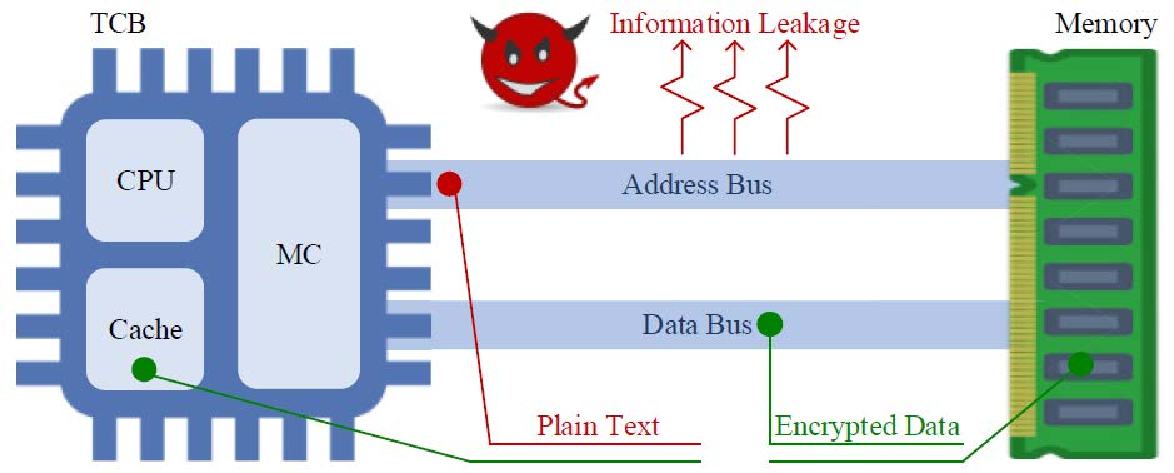
\includegraphics[width=0.8\textwidth]{introduction/leakage.pdf}
    \caption{内存总线上访问模式的泄露}
    \label{fig:leak}
\end{figure}
Goldreich与Ostrovsky在论文中\cite{ref4}提出了不经意随机访问机 (Oblivious RAM, abbr. ORAM)技术。这一技术的目的是隐藏对真实数据块的访问,使得攻击者不能区分每一次访问是真实的还是随机的。不经意随机访问机应用于云存储系统可以有效的防止攻击者利用访问模式获取隐私信息,减小数据存储系统的攻击面,打破了单纯使用传统加密方式来保护数据隐私的系统框架,为用户提供更完善的安全存储服务。\par%
但是,不经意随机访问机也会带来额外的开销,比如:为了隐藏访问模式,需要对多个数据块进行访问,这增大了客户端与服务器之间的带宽,客户端需要更大的缓存空间来存储从服务器端返回的额外数据块。所以,不经意随机访问机的实用性还面临很大的挑战。
\subsection{ORAM安全性定义}\par
为保护和混淆内存的访问模式,ORAM 保证了在存储器中的任意数据块不会永久驻留在某一个物理地址中,这确保了任意两次访问不会产生关联。同时,ORAM将每一次读写访问 (access) 细化成一次读取加一次写回的原子操作 (operation) ,其中读问转化成读取内容再写回相同内容,写访问转化成读取内容再写回更新后的内容,使得攻击者不能够区分具体的访问方式。ORAM能很好地保护
\begin{enumerate}
    \item 访问数据块的位置
    \item 数据块请求的顺序
    \item 对相同数据块的访问频率
    \item 具体的读写访问方式
\end{enumerate}
\par\noindent 下面我们对ORAM的安全性进行正式的定义:
\begin{definition}\textbf{ORAM安全性}
    \newline
    设$\vec{y}$为长度为$M$的一系列数据操作序列,$\vec{y}=(op_1,id_1,block_1),\ldots,(op_M,id_M,block_M)$,$op_i$为读操作$read(id_i)$,其读取标识符为$id_i$的块;或写操作$write(id_i,block_i)$,将新数据$block_i$写入到标识符为$id_i$的块中。如果$op_i=read(id_i)$,那么$block_i=null$。
    \newline
    给定操作序列$\vec{y}$,设其经过ORAM加密后的访问模式为$A(\vec{y})$,该ORAM体制是安全的当期仅当对任意两个相同长度序列$\vec{y}, \vec{y'}$,其访问模式$A(\vec{y}), A(\vec{y'})$计算上不可区分。
\end{definition}\par
为了让读写操作不可区分,标准的解决方案是始终采用“先读后写”的操作,不需要写入的时候通过写入无效信息 (dummy write) 来进行混淆。
\subsection{发展脉络}
不经意随机访问机的概念最早起源于RAM (random access machine)模型,RAM是一种重要的计算仿真手段。在这个模型中,处理器通过对存储器的读写来实现程序的执行。上个世纪80年代,为了隐藏程序对内存的访问模式来避免软件的逆向工程,Goldriche等人在此基础上提出了ORAM\cite{ref2},开启了ORAM的研究历程。不经意随机访问机面临的最大问题是性能开销大。纵观不经意随机访问机的发展。其设计模型大致可以分为5类:简单模型、平方根模型\cite{ref5,ref6}、层次模型\cite{ref5}、分区模型\cite{ref7}和树状模型\cite{ref8,ref9}。不同的设计模型表示服务器存储数据块的数据结构不同,用户通过对服务器ORAM的访问来获取所需的数据块,这些模型设计的目标主要还是提高性能。本文主要介绍后4种模型及其变种,并简介ORAM的最新研究进展。
	\section{Algorithm Specification}
\subsection{Description of Skip List}
The structure of an ordinary ordered Linked List is as follows ($H$ and $T$ refers to the head node and tail node of the list, which contains no valid value):
\begin{figure}[H]
    \centering
    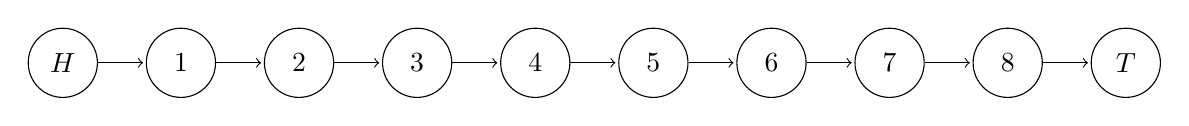
\begin{tikzpicture}[shorten >=1pt,node distance=1.5cm,on grid]
        \node[state] (H)  at (0,0) {$H$};
        \node[state] (n1) at (1.5,0) {$1$};
        \node[state] (n2) at (3,0) {$2$};
        \node[state] (n3) at (4.5,0) {$3$};
        \node[state] (n4) at (6,0) {$4$};
        \node[state] (n5) at (7.5,0) {$5$};
        \node[state] (n6) at (9,0) {$6$};
        \node[state] (n7) at (10.5,0) {$7$};
        \node[state] (n8) at (12,0) {$8$};
        \node[state] (T)  at (13.5,0) {$T$};

        \path[->] (H)  edge [] node []{} (n1)
                  (n1) edge [] node []{} (n2)
                  (n2) edge [] node []{} (n3)
                  (n3) edge [] node []{} (n4)
                  (n4) edge [] node []{} (n5)
                  (n5) edge [] node []{} (n6)
                  (n6) edge [] node []{} (n7)
                  (n7) edge [] node []{} (n8)
                  (n8) edge [] node []{} (T);
    \end{tikzpicture}
    \caption{Ordered Linked List}\label{fig:lkl}
\end{figure}
If we want to find $7$ in the list, we'll have to sequentially search $1\to 2\to \ldots\to 7$, which is $O(N)$. But in an ordered array, we can use binary search to reduce the complexity to $O(\log{N})$. But a linked list doesn't support randomized access, thus we can't use binary search method.\par
A skip list is bulit in levels. If we store some internal nodes in a higher level, we can support a searching method similar to binary search.\\
Now we search 7 again, starting from head node $H$:
\begin{enumerate}
    \item Compare 4 and 7, 7 > 4; compare 8 and 7, 7 < 8, go down at 4
    \item Compare 6 and 7, 7 > 6; compare 8 and 7, 7 < 8, go down at 6
    \item Compare 7 and 7, 7 = 7, found!
\end{enumerate}
The process of finding 7 is as figure \ref{fig:skl}:
\begin{figure}[H]
    \centering
    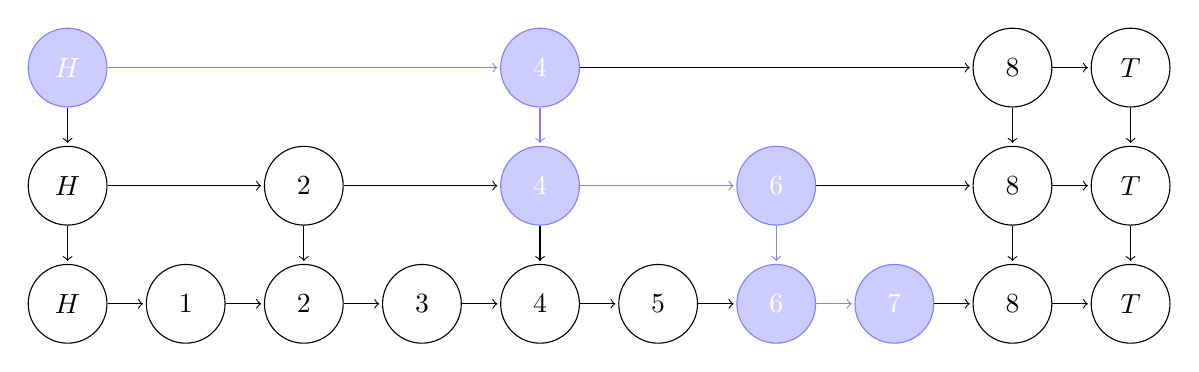
\begin{tikzpicture}[shorten >=1pt,node distance=1.5cm,on grid,
        place/.style={circle,draw=blue!50,fill=blue!20,text=white,minimum size=10mm},
        every state/.style={fill=none,draw=black,text=black,minimum size=10mm}]
        
        \node[place] (H1)  at (0,3) {$H$};
        \node[place] (n11) at (6,3) {$4$};
        \node[state] (n12) at (12,3) {$8$};
        \node[state] (T1) at (13.5,3) {$T$};

        \node[state] (H2)  at (0,1.5) {$H$};
        \node[state] (n21) at (3,1.5) {$2$};
        \node[place] (n22) at (6,1.5) {$4$};
        \node[place] (n23) at (9,1.5) {$6$};
        \node[state] (n24) at (12,1.5) {$8$};
        \node[state] (T2) at (13.5,1.5) {$T$};

        \node[state] (H3)  at (0,0) {$H$};
        \node[state] (n31) at (1.5,0) {$1$};
        \node[state] (n32) at (3,0) {$2$};
        \node[state] (n33) at (4.5,0) {$3$};
        \node[state] (n34) at (6,0) {$4$};
        \node[state] (n35) at (7.5,0) {$5$};
        \node[place] (n36) at (9,0) {$6$};
        \node[place] (n37) at (10.5,0) {$7$};
        \node[state] (n38) at (12,0) {$8$};
        \node[state] (T3)  at (13.5,0) {$T$};

        \path[->] 
                  (H1)  edge [blue!50] node []{} (n11)
                  (n11) edge [] node []{} (n12)
                  (n12) edge [] node []{} (T1)

                  (H2)  edge [] node []{} (n21)
                  (n21) edge [] node []{} (n22)
                  (n22) edge [blue!50] node []{} (n23)
                  (n23) edge [] node []{} (n24)
                  (n24) edge [] node []{} (T2)
        
                  (H3)  edge [] node []{} (n31)
                  (n31) edge [] node []{} (n32)
                  (n32) edge [] node []{} (n33)
                  (n33) edge [] node []{} (n34)
                  (n34) edge [] node []{} (n35)
                  (n35) edge [] node []{} (n36)
                  (n36) edge [blue!50] node []{} (n37)
                  (n37) edge [] node []{} (n38)
                  (n38) edge [] node []{} (T3)
                  
                  (H1)  edge [] node []{} (H2)
                  (H2)  edge [] node []{} (H3)
                  
                  (n21)  edge [] node []{} (n32)
                  
                  (n11)  edge [blue!50] node []{} (n22)
                  (n22)  edge [] node []{} (n34)
                  
                  (n23)  edge [blue!50] node []{} (n36)

                  (n12)  edge [] node []{} (n24)
                  (n24)  edge [] node []{} (n38)
                  
                  (T1)  edge [] node []{} (T2)
                  (T2)  edge [] node []{} (T3);
    \end{tikzpicture}
    \caption{Structure of Skip List and the search path of finding 7}\label{fig:skl}
\end{figure}
In other words, skip list stores some indices of the binary search, which combines the structure of linked list and the method of binary search.

\subsection{Data Structure of skip list}
Firstly, we define the structure of nodes in the skip list:
\begin{lstlisting}[language={C++}]
struct SkipListNode {
    int value;
    int level;
    SkipListNode **next_nodes;
};
\end{lstlisting}
\texttt{value} refers to the value in the node, and \texttt{level} refers to the level. The difference between our implementation of skip list and ordinary linked list is that we store the successor nodes in an array, so that the same node in different levels shares the same storage space. \texttt{next\_nodes[i]} is the successor node in level \texttt{i}. For example, for the node $4$ in figure \ref{fig:skl}, \texttt{next\_nodes[0]} is $5$, \texttt{next\_nodes[1]} is $6$, and \texttt{next\_nodes[2]} is $8$. In this way, we can decrease the space complexity and reduce the structure in figure \ref{fig:skl} to as follows:
\begin{figure}[H]
    \centering
    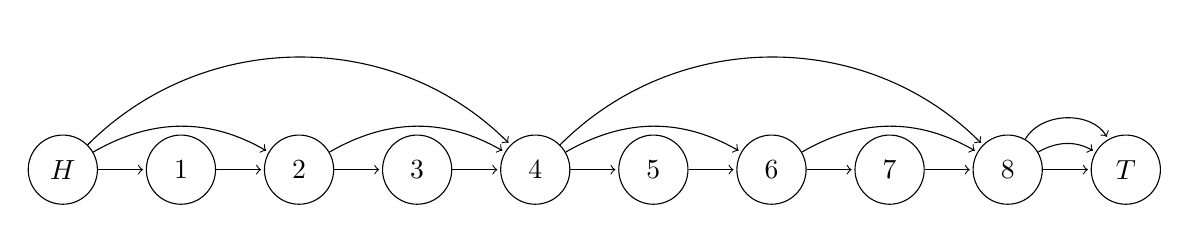
\begin{tikzpicture}[shorten >=1pt,node distance=1.5cm,on grid]
        \node[state] (H)  at (0,0) {$H$};
        \node[state] (n1) at (1.5,0) {$1$};
        \node[state] (n2) at (3,0) {$2$};
        \node[state] (n3) at (4.5,0) {$3$};
        \node[state] (n4) at (6,0) {$4$};
        \node[state] (n5) at (7.5,0) {$5$};
        \node[state] (n6) at (9,0) {$6$};
        \node[state] (n7) at (10.5,0) {$7$};
        \node[state] (n8) at (12,0) {$8$};
        \node[state] (T)  at (13.5,0) {$T$};

        \path[->] (H)  edge [] node []{} (n1)
                  (H)  edge [bend left] node []{} (n2)
                  (H)  edge [bend left = 45] node []{} (n4)
                  (n1) edge [] node []{} (n2)
                  (n2) edge [] node []{} (n3)
                  (n2) edge [bend left] node []{} (n4)
                  (n3) edge [] node []{} (n4)
                  (n4) edge [] node []{} (n5)
                  (n4) edge [bend left] node []{} (n6)
                  (n4) edge [bend left = 45] node []{} (n8)
                  (n5) edge [] node []{} (n6)
                  (n6) edge [] node []{} (n7)
                  (n6) edge [bend left] node []{} (n8)
                  (n7) edge [] node []{} (n8)
                  (n8) edge [] node []{} (T)
                  (n8) edge [bend left] node []{} (T)
                  (n8) edge [bend left = 60] node []{} (T);
    \end{tikzpicture}
    \caption{Skip List with shared nodes}\label{fig:skl2}
\end{figure}
Then, we define the structure of the skip list:
\begin{lstlisting}[language=C++]
class SkipList {
    public:
        SkipList(int max_level); //Constructor
        void Insert(int value);
        void Delete(int value);
        SkipListNode *Find(int value);
        void show(); //to print the list
    private:
        int Max_Level;
        SkipListNode *head;
        SkipListNode *tail;
        static int random_level(int max); //Determine the level of a node randomly
};
\end{lstlisting}

\subsection{Operations on skip list}

\subsubsection{Search}
A brief description of search is shown by a specific case in the last section. Now let's introduce it formally.\par
\begin{enumerate}
    \item Start at the $node = H$ and $level = max\_level - 1$
    \item Move ahead to next node until tail or $value \leq node.value$
    \item If $value = node.value$ return $node$, else $level = level - 1$ and repeat step 2
    \item If $level = 0$ and still not found, return $null$
\end{enumerate}
In pseudo-code:
\begin{algorithm}[H]
    \caption{Skip List: Find}
    \begin{algorithmic}[1]
		\Procedure {find}{$value$}
            \State $node \gets H$
            \For{$level \gets max\_level - 1 \ \mathbf{to}\ 0$}
                \While{$node.next\_nodes[level] \neq T\ \ {\rm and}\ \ node.value < value$}
                    \State $node \gets node.next\_nodes[level]$
                \EndWhile
                \If{$node.value = value$}
                    \State \Return $node$
                \EndIf
            \EndFor
            \State \Return $null$
		\EndProcedure
	\end{algorithmic}
\end{algorithm}

\subsubsection{Insertion}
There are 3 steps when we insert a new value into a skip list: finding the predecessors, creating a new node and finally insert into the list:
\begin{enumerate}
    \item Finding the predecessors:\\
          Firstly, we need to locate the position of the newly-inserted node in the list by finding its predecessors. This step is similar to the find operation, just to find the last node whose value is less than the new value in each level.
    \item Creating a new node:\\
          In this step, we construct a new node and choose a number $k$ with a randomized strategy (which will be mentioned below) as the number of levels of the node.
    \item Inserting into the list:\\
          For level $0$ to $k$, insert the new node after its predecessor just like ordinary linked list.
\end{enumerate}
In pseudo-code:
\begin{algorithm}[H]
    \caption{Skip List: Insert}
    \begin{algorithmic}[1]
        \Procedure {insert}{$value$}
            \State{//Step 1: Finding the predecessors}
            \State $predecessors \gets \mathbf{new}\ Node[Max\_level]$
            \State $node \gets H$
            \For{$level \gets max\_level - 1 \ \mathbf{to}\ 0$}
                \While{$node.next\_nodes[level] \neq T\ \ {\rm and}\ \ node.value < value$}
                    \State $node \gets node.next\_nodes[level]$
                \EndWhile
                \State $predecessors[level] \gets node$
            \EndFor
            \State{//Step 2: Creating a new node}
            \State$k \gets$ \Call{random\_level}{$Max\_level$}
            \State $new\_node \gets \mathbf{new}\ Node(value, k)$
            \State{//Step 3: Inserting into the list}
            \For{$level \gets 0 \ \mathbf{to}\ k$}
                \State Insert $new\_node$ after $predecessors[level]$
            \EndFor
		\EndProcedure
	\end{algorithmic}
\end{algorithm}
For example, if we want to insert $9$ into the list in figure \ref{fig:skl2}, and suppose we get $k=2$, then the process is as follows (blue nodes and arrows denotes the search path to locate the predecessor, yellow node is the predecessor, red node denotes the new node. Dashed arrows and red thick arrows denote the old and updated ``next'' relations):
\begin{figure}[H]
    \centering
    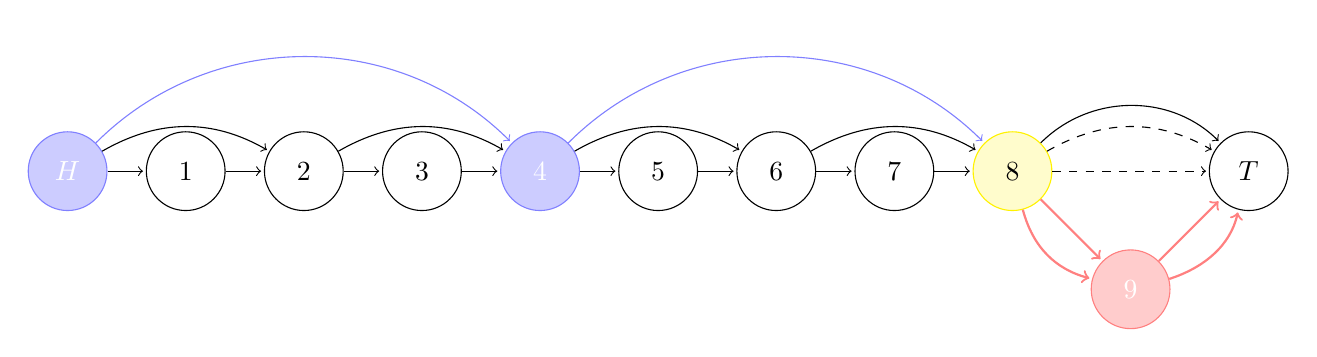
\begin{tikzpicture}[shorten >=1pt,node distance=1.5cm,on grid,
        place/.style={circle,draw=blue!50,fill=blue!20,text=white,minimum size=10mm},
        predecessor/.style={circle,draw=yellow,fill=yellow!20,text=black,minimum size=10mm},
        insert/.style={circle,draw=red!50,fill=red!20,text=white,minimum size=10mm},
        every state/.style={fill=none,draw=black,text=black,minimum size=10mm}]
        \node[place] (H)  at (0,0) {$H$};
        \node[state] (n1) at (1.5,0) {$1$};
        \node[state] (n2) at (3,0) {$2$};
        \node[state] (n3) at (4.5,0) {$3$};
        \node[place] (n4) at (6,0) {$4$};
        \node[state] (n5) at (7.5,0) {$5$};
        \node[state] (n6) at (9,0) {$6$};
        \node[state] (n7) at (10.5,0) {$7$};
        \node[predecessor] (n8) at (12,0) {$8$};
        \node[insert] (n9)  at (13.5,-1.5) {$9$};
        \node[state] (T)  at (15,0) {$T$};

        \path[->] (H)  edge [] node []{} (n1)
                  (H)  edge [bend left] node []{} (n2)
                  (H)  edge [bend left = 45, draw = blue!50] node []{} (n4)
                  (n1) edge [] node []{} (n2)
                  (n2) edge [] node []{} (n3)
                  (n2) edge [bend left] node []{} (n4)
                  (n3) edge [] node []{} (n4)
                  (n4) edge [] node []{} (n5)
                  (n4) edge [bend left] node []{} (n6)
                  (n4) edge [bend left = 45, draw = blue!50] node []{} (n8)
                  (n5) edge [] node []{} (n6)
                  (n6) edge [] node []{} (n7)
                  (n6) edge [bend left] node []{} (n8)
                  (n7) edge [] node []{} (n8)
                  (n8) edge [thick, draw = red!50] node []{} (n9)
                  (n8) edge [bend right, thick, draw = red!50] node []{} (n9)
                  (n8) edge [dashed] node []{} (T)
                  (n8) edge [bend left, dashed] node []{} (T)
                  (n8) edge [bend left = 45] node []{} (T)
                  (n9) edge [thick, draw = red!50] node []{} (T)
                  (n9) edge [bend right, thick, draw = red!50] node []{} (T);
    \end{tikzpicture}
    \caption{Process of inserting $9$}\label{fig:sklins}
\end{figure}
\newpage
\subsubsection{Deletion}
The process of deletion is similar to insertion in 2 steps: finding the predecessor and delete the node.
\begin{algorithm}[H]
    \caption{Skip List: Delete}
    \begin{algorithmic}[1]
        \Procedure {delete}{$value$}
            \State{//Step 1: Finding the predecessors}
            \State $predecessors \gets \mathbf{new}\ Node[Max\_level]$
            \State $node \gets H$
            \For{$level \gets max\_level - 1 \ \mathbf{to}\ 0$}
                \While{$node.next\_nodes[level] \neq T\ \ {\rm and}\ \ node.value < value$}
                    \State $node \gets node.next\_nodes[level]$
                \EndWhile
                \If{$node.next\_nodes[level] \neq tail\ \ {\rm and}\ \ node.next\_nodes[level].value = value$}
                    \State $predecessors[level] \gets node$
                \Else
                    \State $predecessors[level] \gets null$
                \EndIf
            \EndFor
            \State{//Step 2: Deleting the node}
            \For{$level \gets 0 \ \mathbf{to}\ k$}
                \State Delete $new\_node$ after $predecessors[level]$
            \EndFor
		\EndProcedure
	\end{algorithmic}
\end{algorithm}
For example, if we want to insert $6$ in the list in figure \ref{fig:skl2}, then the process is as follows (blue nodes and arrows denotes the search path to locate the predecessor, yellow node is the predecessor, red node denotes the new node. Dashed arrows and red thick arrows denote the old and updated ``next'' relations):
\begin{figure}[H]
    \centering
    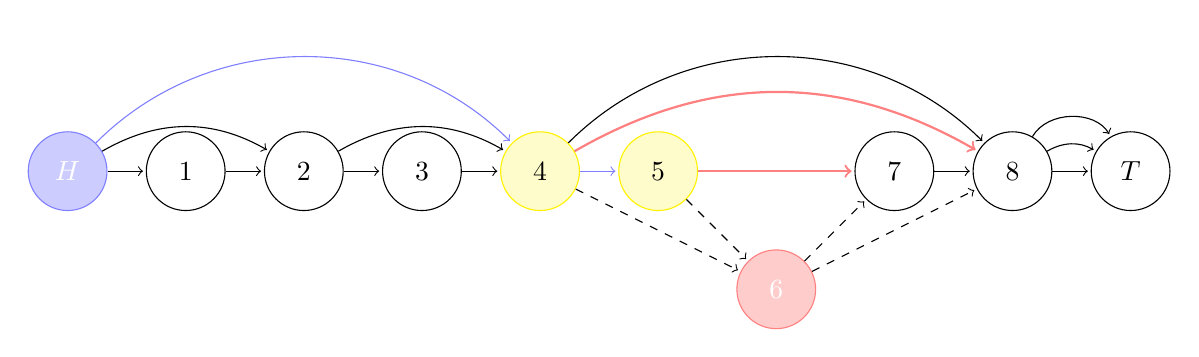
\begin{tikzpicture}[shorten >=1pt,node distance=1.5cm,on grid,
        place/.style={circle,draw=blue!50,fill=blue!20,text=white,minimum size=10mm},
        predecessor/.style={circle,draw=yellow,fill=yellow!20,text=black,minimum size=10mm},
        delete/.style={circle,draw=red!50,fill=red!20,text=white,minimum size=10mm},
        every state/.style={fill=none,draw=black,text=black,minimum size=10mm}]
        \node[place] (H)  at (0,0) {$H$};
        \node[state] (n1) at (1.5,0) {$1$};
        \node[state] (n2) at (3,0) {$2$};
        \node[state] (n3) at (4.5,0) {$3$};
        \node[predecessor] (n4) at (6,0) {$4$};
        \node[predecessor] (n5) at (7.5,0) {$5$};
        \node[delete] (n6) at (9,-1.5) {$6$};
        \node[state] (n7) at (10.5,0) {$7$};
        \node[state] (n8) at (12,0) {$8$};
        \node[state] (T)  at (13.5,0) {$T$};

        \path[->] (H)  edge [] node []{} (n1)
                  (H)  edge [bend left] node []{} (n2)
                  (H)  edge [bend left = 45, draw = blue!50] node []{} (n4)
                  (n1) edge [] node []{} (n2)
                  (n2) edge [] node []{} (n3)
                  (n2) edge [bend left] node []{} (n4)
                  (n3) edge [] node []{} (n4)
                  (n4) edge [draw = blue!50] node []{} (n5)
                  (n4) edge [dashed] node []{} (n6)
                  (n4) edge [bend left, draw = red!50, thick] node []{} (n8)
                  (n4) edge [bend left = 45] node []{} (n8)
                  (n5) edge [dashed] node []{} (n6)
                  (n5) edge [draw = red!50, thick] node []{} (n7)
                  (n6) edge [dashed] node []{} (n7)
                  (n6) edge [dashed] node []{} (n8)
                  (n7) edge [] node []{} (n8)
                  (n8) edge [] node []{} (T)
                  (n8) edge [bend left] node []{} (T)
                  (n8) edge [bend left = 60] node []{} (T);
    \end{tikzpicture}
    \caption{Process of deleting $6$}\label{fig:skldel}
\end{figure}

\subsubsection{Randomization}
Finally, we introduce the random strategy to determine the level $k$ of a new node in the process of insertion.\par
$k$ is a random number between $0$ and $Max\_level$. However, in order to make the expected result to similate binary-search, we don't generate uniform random (i.e. \texttt{k=rand()\%Max\_level}), but make $k$ follows \textbf{Geometric Distribution} with $p = \frac 1 2$. The algorithm is like flipping a coin --- If the coin faces up, the level increases by 1, or else stop at current level:
\begin{algorithm}[H]
    \caption{Random Level}\label{alg:rand}
    \begin{algorithmic}[1]
        \Procedure {random\_level}{}
            \State $level \gets 0$
            \While{$level < Max\_level - 1$}
                \If{$Random\{0,1\}$}
                    \State $level \gets level + 1$
                \Else
                    \State \textbf{break}
                \EndIf
            \EndWhile
            \State\Return{$level$}
		\EndProcedure
	\end{algorithmic}
\end{algorithm}
Suppose the maximum level is $M$, then
\[
    P(k=n)=\left\{
        \begin{aligned}
            &(\frac 1 2)^{n+1},\ n < M-1\\
            &(\frac 1 2)^{n}=(\frac 1 2)^{M-1},\ n = M-1
        \end{aligned}
        \right.
\]
If the size of the skip list is $N$, then the expected number of nodes in the $k_{th}$ level is $E(N_k) = \frac{N}{2^k}$, each level decreases by $\frac 1 2$, just like the process of binary search.
	\section{Testing Results}
In this section, we test the running time of insertion, deletion and searching. We use \texttt{time()} function in C standard library to record the total time of $N$ operations (insertion/deletion/search). For small $N$, the running time is too short (less than 1 ms), we make several iterations of the same operations and compute the average time.\par 
As insertion/deletion will modify the skip list, the size of the skip list will change after each operation. Thus, we only record the total running time of $N$ insertions/deletions, instead of dividing $N$ to get the average time per operation (which is meaningless because the size of the skip list isn't fixed). But for searching, the size of the skip list doesn't change after each operation, so we can divide $N$ to get the average time per operation.
\subsection{Insertion}
In this test, we insert $N$ values from $0$ to $N-1$ into a skip list with $Max\_level=32$ in an order of
\begin{itemize}
    \item Increasing, i.e. $0,1,2,\ldots,N-1$
    \item Decreasing, i.e. $N-1,N-2,\ldots,1$
    \item Random
\end{itemize}
And we record the total time of $N$ insertions. The result is as follows:
\begin{figure}[H]
    \centering
    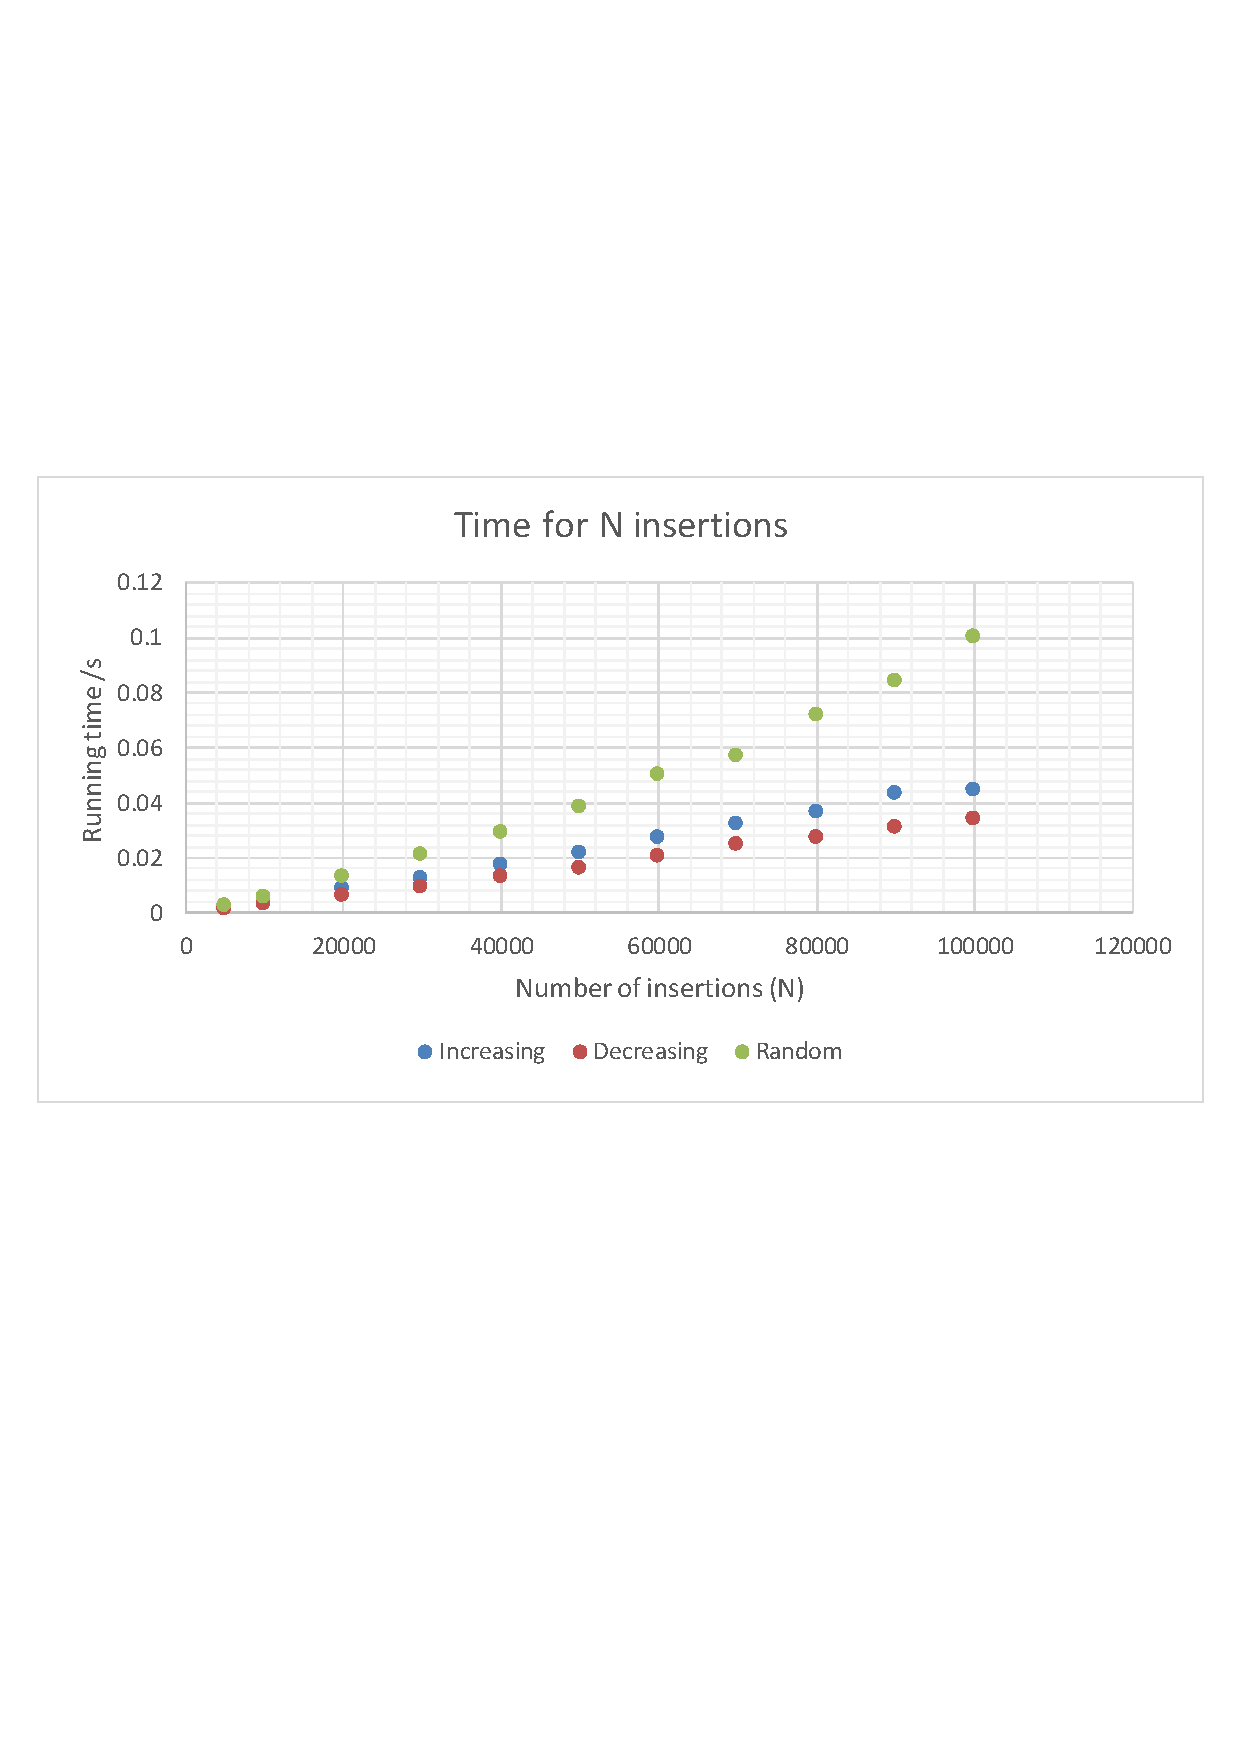
\includegraphics[width=\textwidth]{testing_results/insert.pdf}
    \caption{Running time for 3 insert orders}
\end{figure}

\subsection{Deletion}
We first create a skip list with $Max\_level=32$ and insert $N$ values from $0$ to $N-1$ into it. Then, we delete the values in an order of
\begin{itemize}
    \item Increasing, i.e. $0,1,2,\ldots,N-1$
    \item Decreasing, i.e. $N-1,N-2,\ldots,1$
    \item Random
\end{itemize}
We use the same method as we did in the insertion test to record the total time of $N$ deletions. The result is as follows:
\begin{figure}[H]
    \centering
    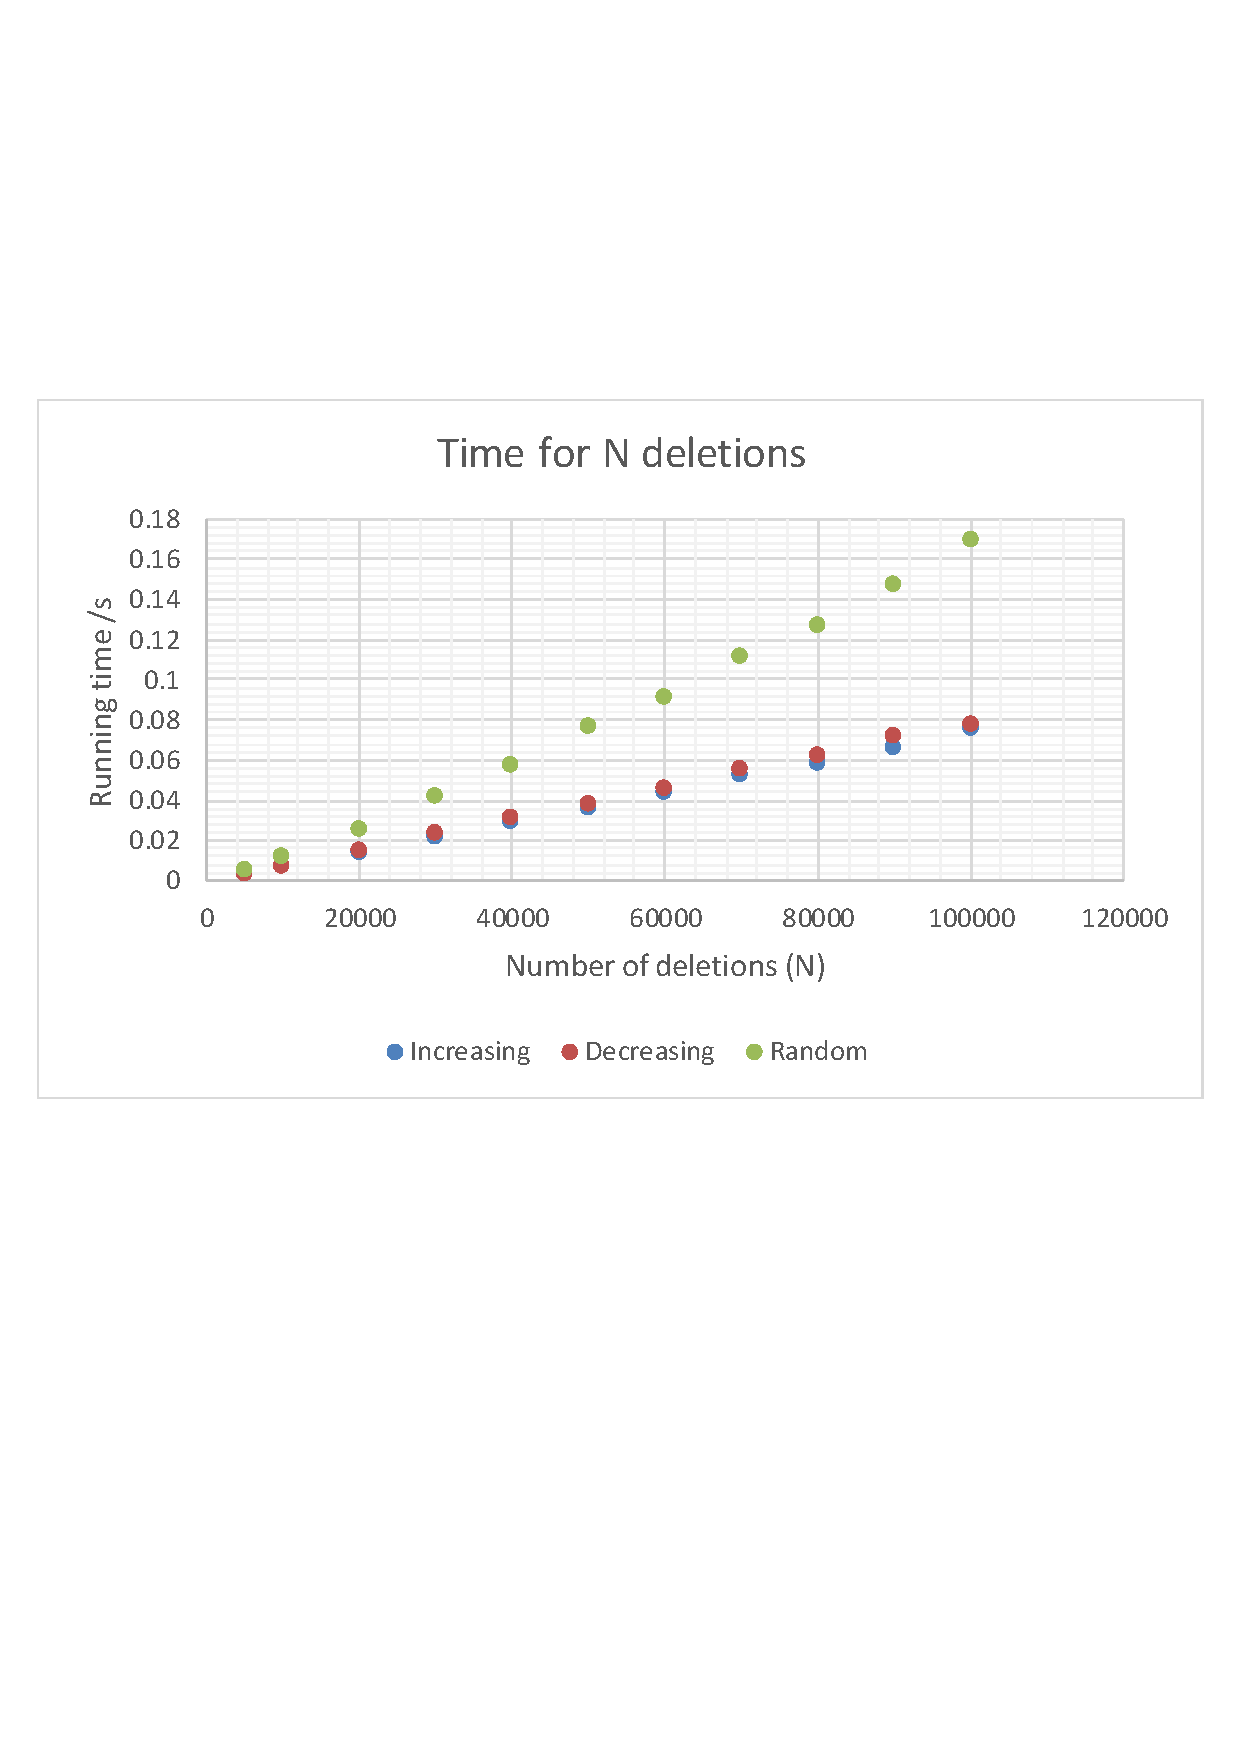
\includegraphics[width=\textwidth]{testing_results/delete.pdf}
    \caption{Running time for 3 delete orders}
\end{figure}

\subsection{Search}
Finally, we test the time of the find operation.\par
We first create a skip list with $Max\_level=32$ and insert $N$ values from $0$ to $N-1$ into it. Then, we find a random value between $[0, N)$ from the skip list for $N$ times. The average time per searching is $\frac{\text{total time}}{N}$. The result is as follows:
\begin{figure}[H]
    \centering
    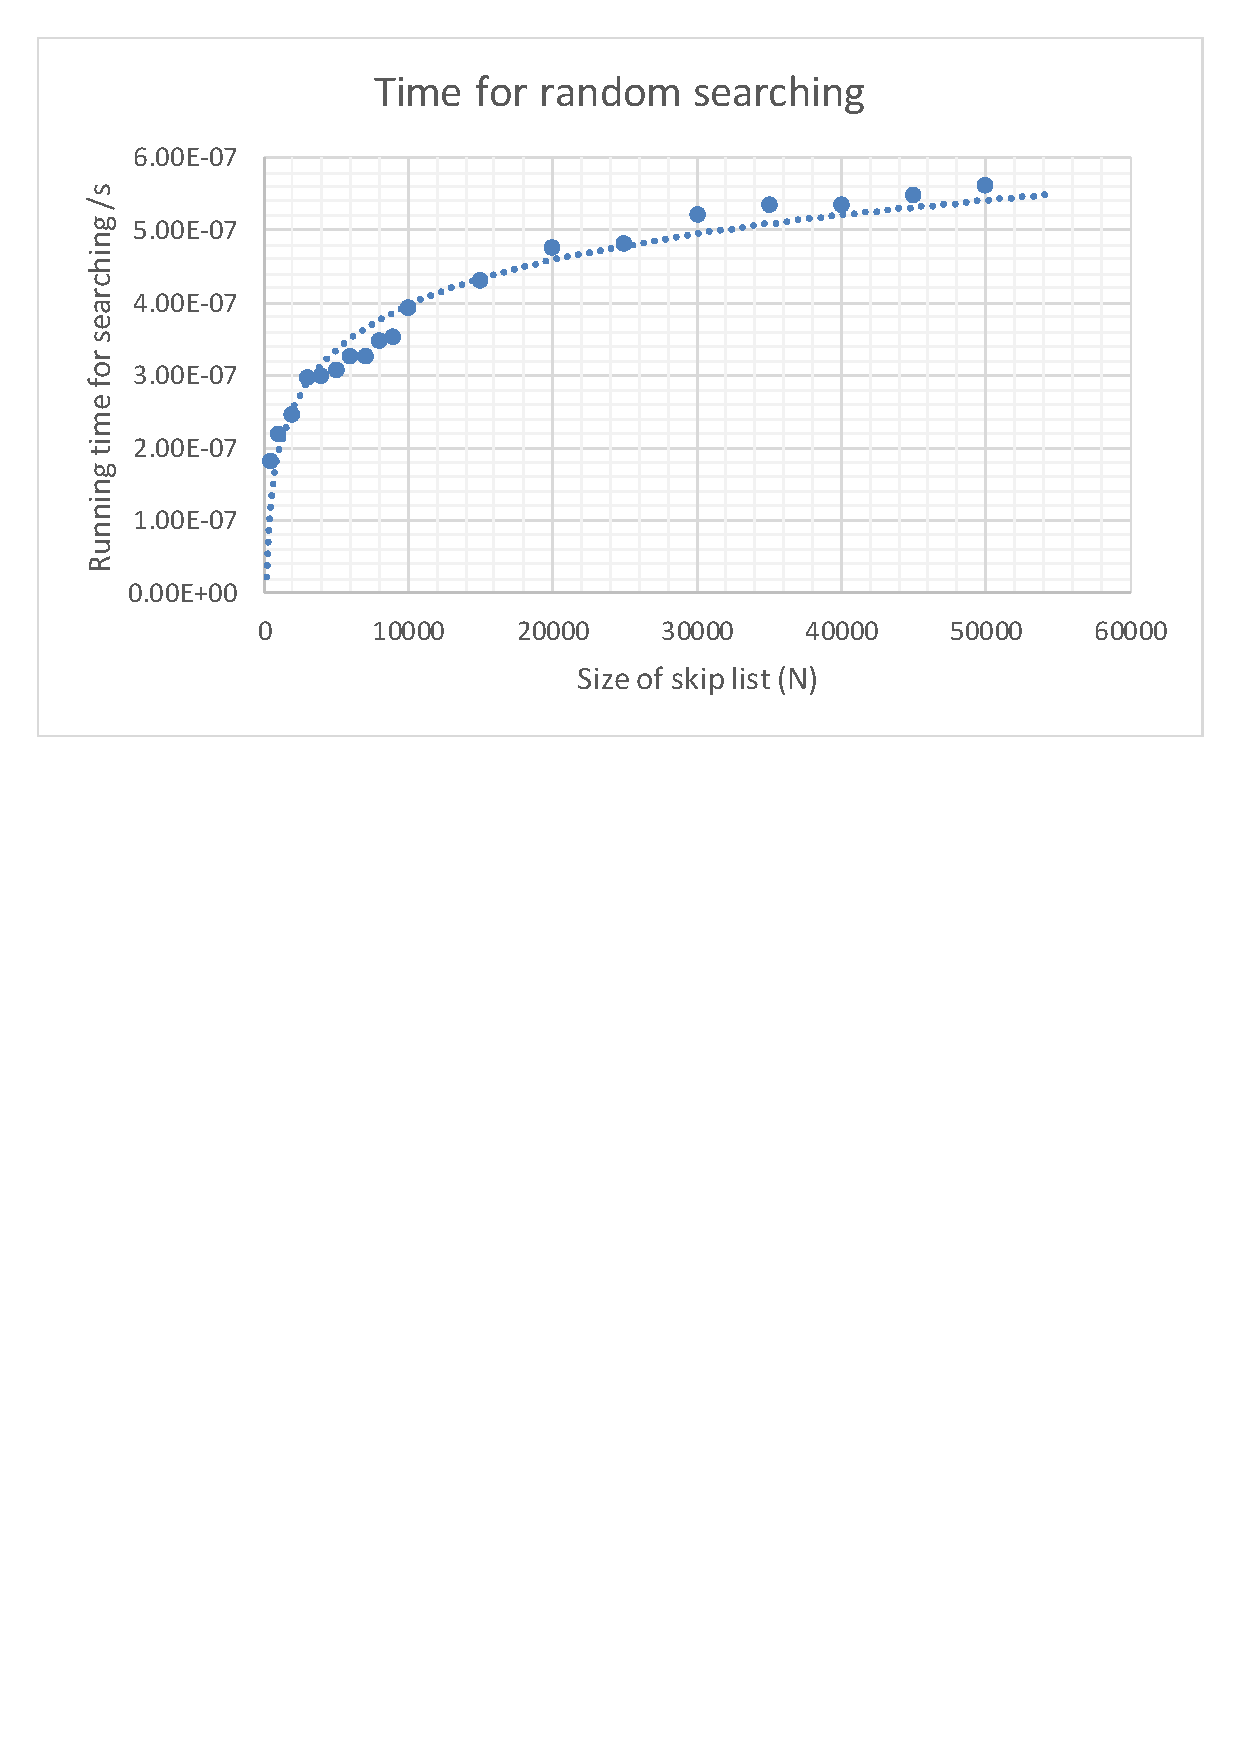
\includegraphics[width=\textwidth]{testing_results/search.pdf}
    \caption{Running time for searching}
\end{figure}
From the figure, we observe that the time complexity of finding seems to be $O(\log{N})$.
	\section{Analysis and Comments}
Because skip list is based on a randomized algorithm, all the complexities analyzed below is the mathematical expectation. The worst-case complexity might be worse, but only with a very small probability.
\subsection{Time Complexity}
In this section, we will prove that the expectation of time complexity of search, insertion and deletion is $O(\log{N})$.
\subsubsection{The expected $Max\_level$}
Let $p$ denotes the probability of increasing the level in the random\_level algorithm \ref{alg:rand} (In our implementation, $p=\frac 1 2$). For an arbitary node, let $k$ denotes the level of it, then $P(k=i)=p^i(1-p)$(i.e. Geometric distribution). Then, the expected number of elements in the $k_{th}$ level (denoted $N_k$) is 
\[
    E(N_k) = \left\{
        \begin{aligned}
            &N,\ k=0\\
            &N(1-\sum_{i=0}^{k-1}p^i(1-p))=N(1-\frac{(1-p)(1-p^k)}{1-p})=Np^k,\ k\geq 1
        \end{aligned}
    \right.
\]
To make the search efficient, we want the highest level $M-1$($M$ is the total number of levels) has an expected $O(1)=a$ number of elements, i.e.
\begin{align*}
    E(N_{M-1})=Np^{M-1}&=a\\
    \log_p{N}+M-1&=\log_p{a}\ \text{(Logarithm on both sides)}\\
    \therefore M=-O(\log_p{N})&=O(\log_\frac{1}{p}N)
\end{align*}
Therefore, the $Max\_level$ of the skip list can be set to $\log_\frac{1}{p}N$ to obtain maximum expected efficiency. In computer, the range of integer is $[0,2^{32})$, so $Max\_level$ is often set to be 32 in practical.
\subsubsection{The expected search cost}
We use a reverse analysis method to analyze the cost. Suppose we have found the node in the $k_{th}$ level, we analyze the search path backwards, going up and left to the head $H$.\par
At an arbitary node $x$ in the $i_{th}$ level in the backward-path, there are 2 situations:
\begin{enumerate}
    \item The level of node $x$ is exactly $i$, then the next step is to go left.\label{enu:case1}
    \item The level of node $x$ is larger than $i$, then the next step is to continue to climb up.\label{enu:case2}
\end{enumerate}
Let's take the case of finding 7 in section 2 as an example. The dashed arrows denote the path backwards. The red 6 and 4 nodes satisfy 2 situations above respectively:
\begin{figure}[H]
    \centering
    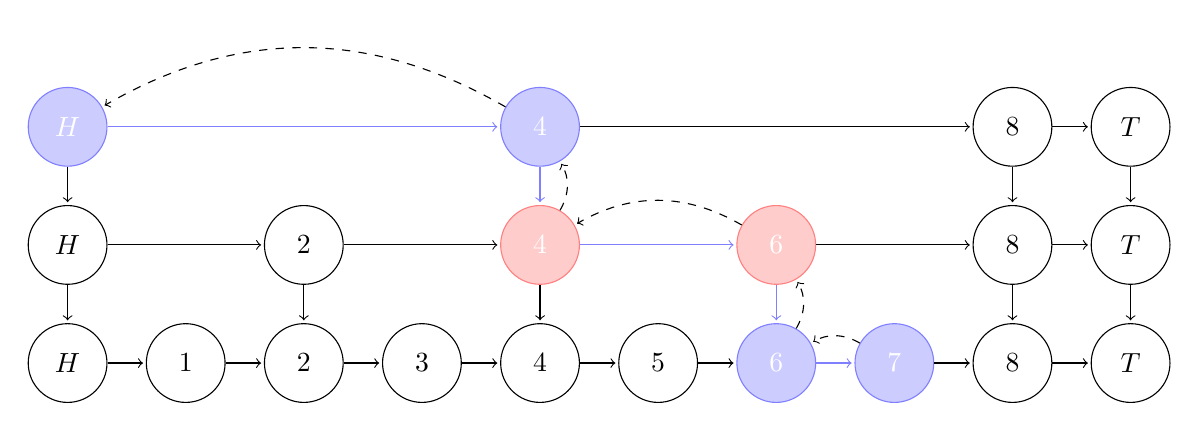
\begin{tikzpicture}[shorten >=1pt,node distance=1.5cm,on grid,
        place/.style={circle,draw=blue!50,fill=blue!20,text=white,minimum size=10mm},
        sit/.style={circle,draw=red!50,fill=red!20,text=white,minimum size=10mm},
        every state/.style={fill=none,draw=black,text=black,minimum size=10mm}]
        
        \node[place] (H1)  at (0,3) {$H$};
        \node[place] (n11) at (6,3) {$4$};
        \node[state] (n12) at (12,3) {$8$};
        \node[state] (T1) at (13.5,3) {$T$};

        \node[state] (H2)  at (0,1.5) {$H$};
        \node[state] (n21) at (3,1.5) {$2$};
        \node[sit] (n22) at (6,1.5) {$4$};
        \node[sit] (n23) at (9,1.5) {$6$};
        \node[state] (n24) at (12,1.5) {$8$};
        \node[state] (T2) at (13.5,1.5) {$T$};

        \node[state] (H3)  at (0,0) {$H$};
        \node[state] (n31) at (1.5,0) {$1$};
        \node[state] (n32) at (3,0) {$2$};
        \node[state] (n33) at (4.5,0) {$3$};
        \node[state] (n34) at (6,0) {$4$};
        \node[state] (n35) at (7.5,0) {$5$};
        \node[place] (n36) at (9,0) {$6$};
        \node[place] (n37) at (10.5,0) {$7$};
        \node[state] (n38) at (12,0) {$8$};
        \node[state] (T3)  at (13.5,0) {$T$};

        \path[->] 
                  (H1)  edge [blue!50] node []{} (n11)
                  (n11) edge [dashed, bend right] node []{} (H1)
                  (n11) edge [] node []{} (n12)
                  (n12) edge [] node []{} (T1)

                  (H2)  edge [] node []{} (n21)
                  (n21) edge [] node []{} (n22)
                  (n22) edge [blue!50] node []{} (n23)
                  (n23) edge [dashed, bend right] node []{} (n22)
                  (n23) edge [] node []{} (n24)
                  (n24) edge [] node []{} (T2)
        
                  (H3)  edge [] node []{} (n31)
                  (n31) edge [] node []{} (n32)
                  (n32) edge [] node []{} (n33)
                  (n33) edge [] node []{} (n34)
                  (n34) edge [] node []{} (n35)
                  (n35) edge [] node []{} (n36)
                  (n36) edge [blue!50] node []{} (n37)
                  (n37) edge [dashed, bend right] node []{} (n36)
                  (n37) edge [] node []{} (n38)
                  (n38) edge [] node []{} (T3)
                  
                  (H1)  edge [] node []{} (H2)
                  (H2)  edge [] node []{} (H3)
                  
                  (n21)  edge [] node []{} (n32)
                  
                  (n11)  edge [blue!50] node []{} (n22)
                  (n22)  edge [dashed, bend right] node []{} (n11)
                  (n22)  edge [] node []{} (n34)
                  
                  (n23)  edge [blue!50] node []{} (n36)
                  (n36)  edge [dashed, bend right] node []{} (n23)

                  (n12)  edge [] node []{} (n24)
                  (n24)  edge [] node []{} (n38)
                  
                  (T1)  edge [] node []{} (T2)
                  (T2)  edge [] node []{} (T3);
    \end{tikzpicture}
    \caption{The search path backwards from 7}\label{fig:back}
\end{figure}
The red node 6 is in level 1, equals to the maximum level of itself, so satisfies case \ref{enu:case1}; while the red node 4 is in level 1 but the maximum level of itself is 2, which satisfies \mbox{case \ref{enu:case2}.}\par
Because the level follows geometric distribution, in an arbitary node $x$, it has a probability of $1-p$ to satisfy case \ref{enu:case1} while $p$ to satisfy case \ref{enu:case2}. Let $C(k)$ denotes the expected cost of search path that climbs up $k$ level, then
\begin{align*}
    C(0) &= 0\\
    C(k) &= (1-p)(1+\text{cost in situation \ref{enu:case2}})+p(1+\text{cost in situation \ref{enu:case1}})\\
    &= (1-p)(C(k)+1) + p(C(k-1)+1)\\
    \therefore C(k) &= \frac{1}{p} + C(k-1)\\
    \therefore C(k) &= \frac{k}{p}
\end{align*}
Because $k\leq Max\_level = O(\log_{\frac 1p}{N})$, thus $C(k)=O(\log{N})$. The time complexity of search is proportional to the cost of the search path, thus we finish the proof that the expected time of search is $O(\log{N})$.
\subsubsection{The expected insertion/deletion cost}
The insertion/deletion takes 2 steps:
\begin{enumerate}
    \item Find the predecessor
    \item Insert/Delete
\end{enumerate}
Step 1 costs $O(\log{N})$ while step 2 costs $O(k)\leq Max\_level = O(\log{N})$ where $k$ is the level of the node to insert/delete, thus the expected time of insertion/deletion is also $O(\log{N})$.

\subsection{Space complexity}
The level $L$ follows geometric distribution, so the expectation of $L$ is
\[
    E(L) = \sum_{k=0}^\infty kp^k(1-p) = \frac{1}{1-p}
\]
For each node, it costs $O(L)$ space to store the successors array \texttt{next\_nodes}. Therefore, the space complexity of a skip list is $O(NL)=O(\frac{N}{1-p})=O(N)$. The smaller $p$ is, the less space the skip list costs.\par
Here, we assume that the maximum level is infinity. If max level is finite (denoted $M$), we have
\[
    P(L=k)=\left\{
        \begin{aligned}
            &p^k(1-p),\ k<M-1\\
            &1-\sum_{k=0}^{M-2}p^k(1-p)=p^{M-1},\ k=M-1
        \end{aligned}
        \right.
\]
When $M=O(\log{N})$ is large, $(M-1)p^{M-1}\to0$, the bias caused by assuming infinity level can be ignored. Thus, for skip list with finite level, the space complexity is still $O(N)$. 

\subsection{Further thinking}
As an emerging data structure, skip list exudes its unique brilliance with its high efficiency and simplicity. Compared to balanced search trees, skip list is not inferior to them.\par
For a long time, in order to optimize the efficiency of searching, a lot of sophisticated tree structures are designed. Despite their efficiency, their large programming complexity is unacceptable. Skip list not only describes the structure itself, but also ``skips'' the stereotype of the ``tree'' structure. As a data structure, skip list has been widely used to describe an ordered set instead of using trees in more and more areas. As a way of thinking, ``skipping the stereotype'' leads mankind to making progress one after another!

	\newpage

	\begin{appendices}
		\section*{Source Code}
		Due to limited space, the complete source code isn't included in this report. You can find the source code in \texttt{skip\_list.cpp}, thanks.
		\section*{Author List}
		\begin{itemize}
			\item Programmer: Tao Hongyu
			\item Tester: Tao Hongyu, Zhu Jingsen
			\item Report Writer: Zhu Jingsen
			\item PPT and Presentation: Tong Xinyuan
		\end{itemize}
		\section*{Declaration}
		\textit{We hereby declare that all the work done in this project titled "Skip Lists" is of our independent effort as a group.}
	\end{appendices}

%	\bibliography{oram}

\end{document}
